%\documentclass{beamer}
\documentclass[handout]{beamer}
\usepackage[utf8]{inputenc}
\usepackage[T1]{fontenc}


\title{Haptic Pattern Representation using Music Technologies}
\date[ISPN ’80]{CIM2014 Berlin. 2014-12-04}
\author[MJC]{Michael Cumming BArch PhD \texttt{mcumming@ocadu.ca}}

\usetheme{MJC}
\setbeamerfont{page number in head/foot}{}
\setbeamertemplate{footline}[frame number]
\setbeamertemplate{caption}[numbered]

%tikz stuff
\usepackage{tikz}
\usepackage{pgf}
\usetikzlibrary{arrows,shapes,automata}
%\usepackage[pgf]{dot2texi}
\usepackage{graphicx}
\usepackage{caption}
\usepackage{subcaption}
\usepackage{float}
\usepackage{natbib}
\usepackage{booktabs, tikz, multicol, float, subcaption}
\usetikzlibrary{arrows}
\usepackage[english]{babel}
\floatplacement{figure}{H}
\floatplacement{table}{H}


%\usepackage[margin={6cm,6cm}]{geometry}
%\usepackage[parfill]{parskip}  %avoid indenting first line of paragraph
%\usepackage{enumitem} 
%\setlist[enumerate]{itemsep=0mm}
%\usepackage{type1cm} % scalable fonts

\begin{document}

\setbeamertemplate{frametitle continuation}[from second]

% Now get rid of all the colours
\setbeamercolor*{bibliography entry title}{fg=black}
\setbeamercolor*{bibliography entry author}{fg=black}
\setbeamercolor*{bibliography entry location}{fg=black}
\setbeamercolor*{bibliography entry note}{fg=black}
% and kill the abominable icon
\setbeamertemplate{bibliography item}{}


%\newcommand{\newCommandName}{text to insert}
%Then you can just use \newCommandName{} in the text
%eg. \NORMAL{}

%tikstyles (used by several figures)
%%%%%%%%%%%%%%%%%%%%
\tikzstyle{figureBox} = [fill=white!20, draw=black, thick,
    rectangle, rounded corners=10pt,inner sep=1cm, inner ysep=1cm]
\tikzstyle{textBox} = [fill=orange!20, draw=black, thick,
    rectangle, rounded corners=10pt, inner sep=1cm, inner ysep=1cm]

\begin{center}
%\TITLE{}
\textbf{Haptic pattern representation using music technologies}\\
%\vspace{2em}
\end{center}

\begin{frame}
\titlepage
\end{frame}

\begin{frame}{Summary}
What is the problem?
\begin{itemize}
\item 
\end{itemize}
\pause

\begin{frame}{Summary of Talk}
Version 1
\begin{itemize}
\item Visual Analytics often involve Big Data Sets
\item Big Data Sets usually involve Distributed Action
\item Distributed Action usually results in Emergent Patterns
\end{itemize}
\pause

\bigskip
Version 2
\begin{itemize}
\item Greg van Alstyne's talk last week mentioned Herbert Simon
\item Herbert Simon was a great influence on my work
\item Herbert Simon's (and my) work may connect obliquely with Visual Analytics
%\item Distributed Action implies \emph{Patterns of Interaction}
\end{itemize}
\end{frame}

\begin{frame}{Introduction}
My background
	\begin{itemize}
	\item Architectural practice (mostly in Toronto and Europe)
	\item Academia (Computational design / Computer-aided design)
	\item Ambitious City (Support for bottom-up urban design)
	\item MGDS-PET project at DFI / OCADU (wearable devices to support transmedia narratives)
	\end{itemize}
\end{frame}

\begin{frame}{Herbert Simon, 1916-2001}
\begin{figure}
\begin{center}
 \includegraphics[width=8cm]{images/herbertSimon01.jpg}
    
  \label{fig:herb}
  \citep{simon1996sciences}
  \caption{Pioneering researcher in Artificial Intelligence, Herbert Simon.}
\end{center}
\end{figure}
\end{frame}

\begin{frame}{Complex Patterns and Generating Mechanisms}
\begin{block}{Question}Do patterns that look complex or organic always involve simpler, lower-level interactions? [flocking birds / like ants on a beach]
\end{block}
\pause

\begin{block}{Question}Does Visual Analytics study emergent, organic patterns, or the simpler behaviours that may have created them?
\end{block}
\end{frame}
	
\begin{frame}{Collaborative Design as a type of Distributed Activity}
Design is usually done collaboratively.
\bigskip

\begin{frame}{Thanks for attending!}
\bigskip
Michael Cumming
\texttt{mcumming@ocadu.ca}
\end{frame}

\setlength{\columnsep}{2cm}
\begin{multicols}{2}

\begin{center}
%\BIG{}
\textbf{Michael Cumming, Adam Tindale, Sara Diamond\\
OCAD University, Toronto, Canada}\\
mcumming@ocadu.ca,
atindale@faculty.ocadu.ca,
sdiamond@ocadu.ca\\
\end{center}
\vspace{1em}

\begin{figure}[H] \centering
\includegraphics[width=0.005\textwidth]{graphicsPoster/OCAD_Logo.png}
\end{figure}
%\vspace{-2em}

%\NORMAL{}
We are developing a wrist-wearable, quasi-musical device with vibrotactile arrays, which integrates with a transmedia gaming app on an accompanying smartphone. The main purpose of the wrist device is to register hand gestures and provide clues and notifications for the game player. The vibrotactile arrays also provide pleasant sensual stimulation. We propose that standard musical notation is an appropriate way to program activation patterns for these arrays in a standardized way.\\

%TEXT BOX What is the Problem?
\begin{center}

%\SECTION{}
\textbf{What is the problem?}
%\BIG{}
\begin{itemize}
\item How to author interesting and functional vibrating patterns for devices with low resolution \textit{vibrotactile} arrays
\item How to align these patterns with the configuration of the device
\end{itemize}

\end{center}
\vspace{2em}


\begin{figure}%[H]
\centering
\includegraphics[width=0.15\textwidth]{graphics/bracelet-02.png}
%caption{Bracelet design with 2x5 tactor array.}
\end{figure}
%\vspace{-1em}
\begin{center}
%\NORMAL{}
\textbf{Vibrotactile band with a 2x5 vibe motor array.}
\end{center}


%TEXT BOX Why do this?
\begin{center}
\begin{tikzpicture}
\node [textBox] (box){ % or figureBox
\begin{minipage}{0.45\textwidth}
%\SECTION{}
\textbf{Why do this?}
%\BIG{}
\begin{itemize}
\item Notification and stimulation from such bands could enrich transmedia narratives and gaming experiences 
\item Touch, vibration and rhythm are important sensual modalities
\item Authoring rhythmic patterns using music notation is efficient and has a long history


\end{itemize}
\end{minipage}};
\end{tikzpicture}
\end{center}
%\vspace{-2em}

%TEXT BOX
\begin{center}
\begin{tikzpicture}
\node [textBox] (box){ % or figureBox
\begin{minipage}{0.45\textwidth}
%\SECTION{}
\textbf{Results}
\BIG{}
\begin{itemize}
\item Standard music notation is typically two-dimensional: x-axis handles time, y-axis is pitch (and z-axis is unused)
\item Physical adjacencies of musical instruments are usually not represented in their notation, therefore, authoring for 2D arrays is not straightforward. Multiplication of parts and staves seems the simplest [naive] approach 
\item Standard music notation provides a nuanced, graphical representation for rhythmic events, which is hugely useful for our purposes.
\end{itemize}
\end{minipage}};
\end{tikzpicture}
\end{center}
%\vspace{-2em}


%\NORMAL{}
\textbf{Acknowledgements}\\
%\SMALL{}
This work has been supported by the International Science and Technology Partnerships Canada Inc (ISTP) on the project \textit{Multi-platform Game Distribution System for Popular and Experimental Technologies} (MGDS-PET) and by grants from the National Sciences and Engineering Research Council of Canada (NSERC). We would also like to thank Xenophile Media Inc., Vicki Clough, Shin-you Hou, Tegan Power, Ryan Maksymic and Takis Zourntos for the their help in the development of this project.\\
%\vspace{-2em}
\begin{figure}[H] \centering
\includegraphics[width=0.1\textwidth]{graphics/ISTP_logo.png}
\hspace{2em}
\includegraphics[width=0.1\textwidth]{graphics/nserc_logo_color.png}
\end{figure}


%ZERO DIM
\begin{center}
\begin{tikzpicture}
\node [figureBox] (box){ % or textBox
\begin{minipage}{0.45\textwidth}
\begin{center}
%\BIGRED{} 
\textbf{Device with no spatial dimension (0D = point)}\\

\vspace{1em}
%\SMALL{}
\begin{tikzpicture}[scale=2]
%grid
\draw[step=1cm,gray,very thin] (0,0) grid (1,1);
%circles:
\filldraw[fill=blue, draw=black] (0.5,0.5) circle (0.12cm);
%\draw[very thin] (0.5,0.5) circle (0.2cm);
%\draw[very thin] (0.5,0.5) circle (0.35cm);
\end{tikzpicture}\\
\textbf{Device with a single vibe motor}

\vspace{1cm}
%bottom figure (musical staff)
\begin{figure}[H] \centering
        \includegraphics[width=0.65\textwidth]{graphicsPoster/arrowsMoving-00.pdf}
\end{figure}
\textbf{Score for single vibe motor playing a simple `solo' rhythm}\\
\end{center}

\begin{itemize}
\item Time = horizontal axis; rhythmic information as per standard musical notation
\item For most vibe motors pitch remains constant, but intensity can vary; Intensity specified by dynamics markings
\item Vertical position does not vary (y-axis unused, therefore unpitched notation would also be suitable)
\item Information is not very dense (single line score would suffice)
\item \textbf{NEXT STEP} notate for multiple vibe motors
\end{itemize}
\rule{\textwidth}{0.5pt}\\

%ONE DIM, unpitched
\begin{center}
%\BIGRED{} 
\textbf{Device with one spatial dimension (1D = linear)}\\
\textbf{Vertical note position maps to five components}\\
\vspace{1em}

%\SMALL{}
%top diagram
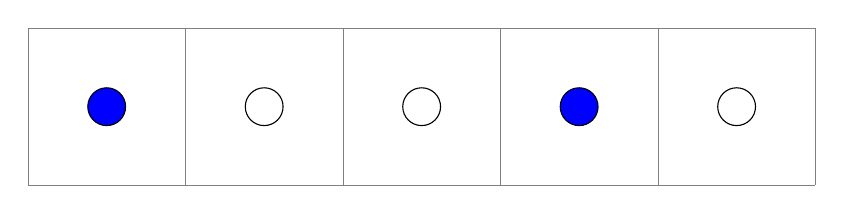
\begin{tikzpicture}[scale=2]
%grid
\draw[step=1cm,gray,very thin] (0,0) grid (5,1);
%bottom row:
\filldraw[fill=blue, draw=black] (0.5,0.5) circle (0.12cm);
\filldraw[fill=white, draw=black] (1.5,0.5) circle (0.12cm);
\filldraw[fill=white, draw=black] (2.5,0.5) circle (0.12cm);
\filldraw[fill=blue, draw=black] (3.5,0.5) circle (0.12cm);
\filldraw[fill=white, draw=black] (4.5,0.5) circle (0.12cm);
\end{tikzpicture}\\
\textbf{Device with a line of vibe motors}.
\vspace{2cm}
%bottom figure (musical staff)
\begin{figure}[H] \centering
        \includegraphics[width=0.8\textwidth]{graphicsPoster/arrowsMoving-00-drumStaff.pdf}
\end{figure}
\textbf{Score for a linear array of five vibe motors}
\end{center}

\begin{itemize}
\item Specifies activations for five, independent vibe motors
\item Each part occupies one staff line (rests are hidden); for unpitched components yet uses five staff lines
\item Vertical staff position specifies vibe motor to activate; top line=1, second line=2, etc; MIDI note $\Rightarrow$ vibe motor
\item \textbf{PROBLEM} Five unpitched parts on one staff are hard to read, especially if rhythms are complex
\item \textbf{NEXT STEP} Make notation less dense and more readable
\end{itemize}
\rule{\textwidth}{0.5pt}\\

%ONE DIM, low density
%bottom figure (musical staff)
\begin{center}
%\BIGRED{}
\textbf{Part numbering maps to five components}\\
\vspace{1em}

%\SMALL{}
\begin{figure}[H] \centering
        \includegraphics[width=0.55\textwidth, height=.35\textwidth]{graphicsPoster/arrowsMoving-01-drumStaves.pdf}
\end{figure}
\textbf{Score for a linear array of five vibe motors}
\end{center}
\begin{itemize}
\item Specifies activations for five, independent components
\item Five part single-line staff, rhythmic notation 
\item MIDI number derived from part number; this maps to vibe motor address
\item \textbf{NEXT STEP} Make notation suitable for two dimensional arrays of vibe motors
\end{itemize}
\rule{\textwidth}{0.5pt}\\

%TWO DIM
\begin{center}
%\BIGRED{} 
\textbf{Device with two spatial dimension (2D = planar)}\\
\vspace{1em}

%\SMALL{}
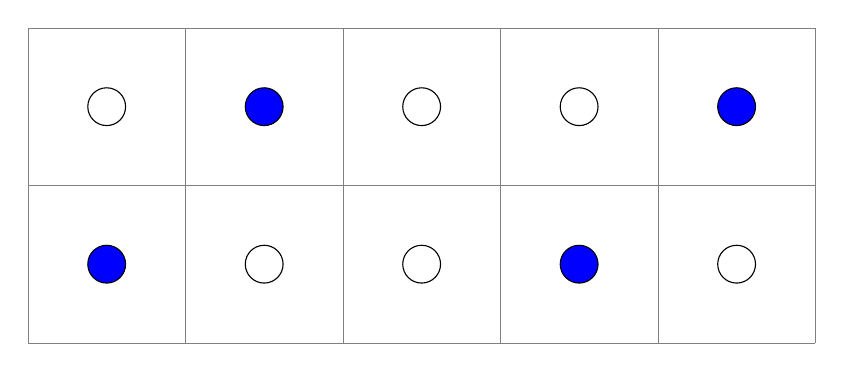
\begin{tikzpicture}[scale=2]
%grid
\draw[step=1cm,gray,very thin] (0,0) grid (5,2);
%top row:
\filldraw[fill=white, draw=black] (0.5,1.5) circle (0.12cm);
\filldraw[fill=blue, draw=black] (1.5,1.5) circle (0.12cm);
\filldraw[fill=white, draw=black] (2.5,1.5) circle (0.12cm);
\filldraw[fill=white, draw=black] (3.5,1.5) circle (0.12cm);
\filldraw[fill=blue, draw=black] (4.5,1.5) circle (0.12cm);
%bottom row:
\filldraw[fill=blue, draw=black] (0.5,0.5) circle (0.12cm);
\filldraw[fill=white, draw=black] (1.5,0.5) circle (0.12cm);
\filldraw[fill=white, draw=black] (2.5,0.5) circle (0.12cm);
\filldraw[fill=blue, draw=black] (3.5,0.5) circle (0.12cm);
\filldraw[fill=white, draw=black] (4.5,0.5) circle (0.12cm);
\end{tikzpicture}\\
\textbf{Device with an array of vibe motors}
\vspace{2cm}

%top score (musical staff)
\begin{figure}[H] \centering
        \includegraphics[width=0.55\textwidth]{graphicsPoster/arrowsMoving-5sysx2lines.pdf}
\end{figure}
\textbf{Score where each staff represents one COLUMN of vibe motors}
\vspace{1em}
%bottom scale (musical staff)
\begin{figure}[H] \centering
        \includegraphics[width=0.6\textwidth]{graphicsPoster/arrowsMoving-2sysx5lines.pdf}
\end{figure}
\textbf{Score where each staff represents one ROW of vibe motors}
\end{center}

\begin{itemize}
\item Time = horizontal, x-axis
\item Ten components need independent addressability 
\item Either five staves (for columns) or two staves (for rows)
\end{itemize}
\end{minipage}};
\end{tikzpicture}
\end{center}



\end{document}